\chapter{Razvojni sustav ESP32-C3-DevKitM-1}

Razvojni sustav temelji se na modulu ESP32-C3-MINI-1. Modul je jedan u nizu ESP32-­C3 serije SoC (engl. \textit{System on Chip}) platformi tvrtke \textit{Espressif}, te sadrži jednojezgreni 32-bitni procesor s RISC-V arhitekturom koji radi na frekvenciji do 160 MHz. Modul sadrži 400 KB memorije tipa SRAM (engl. \textit{Static random-access memory}), od kojih je 16 KB rezervirano za priručnu memoriju (engl. \textit{cache}), 384 MB memorije tipa ROM (engl. \textit{Read-only memory}) te 4 MB memorije tipa \textit{Flash}. Od periferije sadrži 22 programabilna GPIO pina (engl. \textit{General Purpose Input Output}), te digitalna sučelja SPI, UART, I2C i I2S. Također sadrži upravljače za sučelja USB i JTAG koji se mogu koristiti za efikasnije otklanjanje pogrešaka u kodu (engl. \textit{debugging}). \cite{esp32manual} Konfiguracija sustava prikazana je na slici \ref{fig:esp32}.

\begin{figure}[ht]
	\centering
	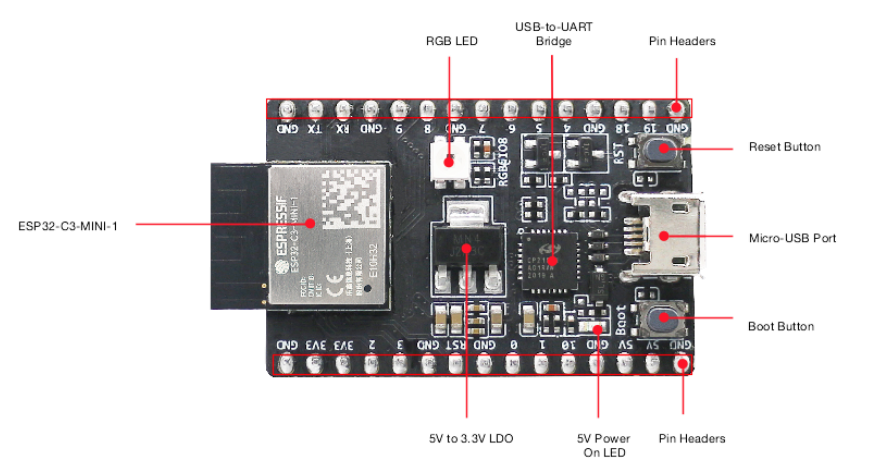
\includegraphics[scale=0.6]{imgs/esp32}
	\caption{Konfiguracija razvojnog sustava ESP32-C3-DevKitM-1 \cite{espressif}}
	\label{fig:esp32}
\end{figure}

Budući da modul ima funkciju RF (engl. \textit{radio frequency}) primopredajnika, podržava bežično lokalno umrežavanje odnosno Wi-Fi, koji omogućava propusnost do 20 Mbps protokolom TCP te maksimalnu propusnost od 30 Mbps koristeći protokol UDP. Isto tako, podržava protokol Bluetooth s podrškom za velike udaljenosti. 

Modul ESP32-C3-MINI-1 bežični je uređaj niske potrošnje energije (engl. \textit{ultra-low-power}) primarno namijenjen razvoju aplikacija koje koriste Wi-Fi ili \textit{Bluetooth Low Energy} (BLE) protokol. Na slici \ref{fig:esp32block} nalazi se blok shema modula sa svim dostupnim značajkama. 

\begin{figure}[ht]
	\centering
	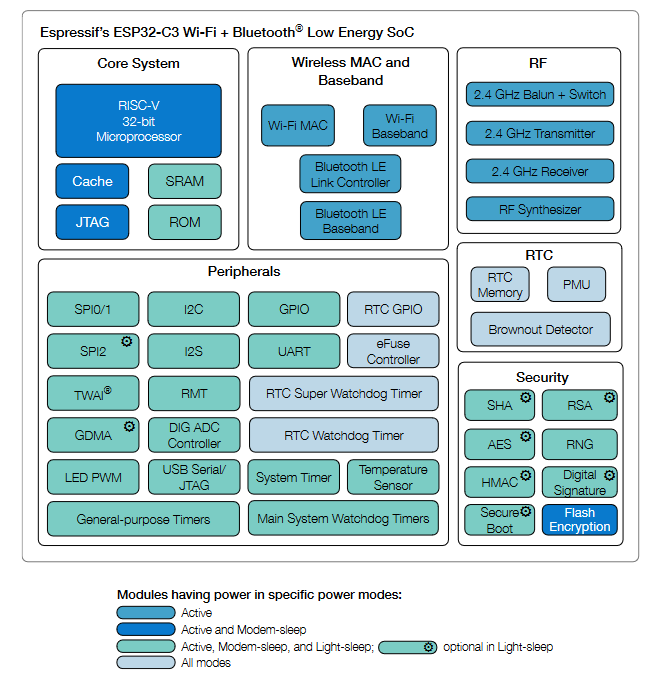
\includegraphics[scale=0.6]{imgs/esp32block}
	\caption{Blok dijagram modula ESP32-C3 \cite{esp32manual}}
	\label{fig:esp32block}
\end{figure}

\section{Wi-Fi}

Podsustav modula za Wi-Fi u skladu je sa standardom IEEE 802.111 te koristi nelicencirani pojas frekvencija na 2,4 GHz. U tom pojasu podržava propusnost od 20 i 40 MHz. Modul također podržava tehniku raznolikosti antena (engl. \textit{antenna diversity}) za poboljšanje prijema i pouzdanosti signala korištenjem RF komutatora (engl. \textit{switch}). Tim komutatorom upravljaju GPIO priključci i koristi se za odabir najbolje antene u kontekstu pouzdanosti i kvalitete signala. 

ESP32-C3 u potpunosti implementira 802.11 b/g/n Wi-Fi MAC protokol. Podržava osnovni skup (engl. \textit{Basic Service Set - BSS}) operacija za značajke pristupne točke (engl. \textit{SoftAP}). Upravljanje napajanjem odvija se automatski s minimalnom intervencijom domaćina kako bi se smanjila aktivnost uređaja.

Tvrtka \textit{Espressif} također nudi biblioteke za povezivanje putem protokola TCP i IP te korištenje Wi-Fi \textit{mesh} tehnologije. Pruža i podršku za protokole TLS 1.0, 1.1 i 1.2. Na slici \ref{fig:wifi_rf_table} prikazani su Wi-Fi RF standardi koje koristi modul. 

\begin{figure}[ht]
	\centering
	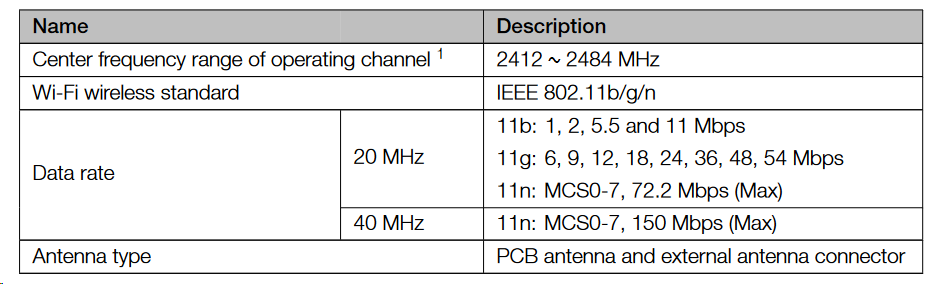
\includegraphics[scale=0.6]{imgs/wifi_rf_table}
	\caption{Wi-Fi RF standardi \cite{esp_mini}}
	\label{fig:wifi_rf_table}
\end{figure}

Wi-Fi MAC automatski primjenjuje sljedeće funkcije protokola niske razine:
\begin{itemize}
	\item četiri virtualna Wi-Fi sučelja,
	\item 
	\item 
	\item 
	\item 
	\item 
	\item 
\end{itemize}


\section{Aplikacijska programska sučelja}

 

\eject